\documentclass[a4paper, 8pt, twoside, openright]{book}
\usepackage[a4paper,top=4cm,bottom=2cm,left=2cm,right=2cm]{geometry}
\usepackage[english]{babel}
\usepackage[T1]{fontenc}
\usepackage[utf8]{inputenc}
\usepackage{fancyhdr}
\usepackage{float}
\usepackage{graphicx}
\usepackage{wrapfig}
\usepackage{siunitx} %per scrivere il simbolo °
\usepackage{verbatim} %per i commenti1
\usepackage{subfig}
\usepackage{amsmath}
\usepackage{algorithm}
\usepackage{algpseudocode}
\setcounter{secnumdepth}{3}
\setcounter{tocdepth}{6}
\usepackage{multirow}
\newcommand{\minitab}[2][l]{\begin{tabular}#1 #2\end{tabular}}
\usepackage{rotating}
\usepackage{xfrac}

\DeclareMathOperator*{\argmax}{arg\,max}
\DeclareMathOperator*{\argmin}{arg\,min}

%\usepackage{booktabs,array}
%\usepackage{tikz}

%\usepackage{tabularx}

%\usepackage{chngcntr}
%\counterwithin{table}{section}

%------------------------------ colors
\usepackage[usenames,dvipsnames,table]{xcolor} % use colors on table and more
\definecolor{333}{RGB}{51, 51, 51} % define custom color
\definecolor{background}{RGB}{248, 248, 255}
\definecolor{comment}{RGB}{17,167,5}
\definecolor{keyword}{RGB}{195,47,8}
\definecolor{string}{RGB}{142,195,0}
\definecolor{number}{RGB}{90,84,84}
\definecolor{identifier}{RGB}{0,90,201}

%------------------------------ source code
\usepackage{listings}

\lstset{
  basicstyle=\footnotesize\sffamily,
  commentstyle=\itshape\color{gray},
  captionpos=b,
  frame=shadowbox,
  language=HTML,
  rulesepcolor=\color{333},
  tabsize=2
}

\lstdefinestyle{code}{
  backgroundcolor=\color{background},
  basicstyle=\footnotesize\sffamily,
  commentstyle=\color{comment},
  frame=L,
  identifierstyle=\color{identifier},
  keywordstyle=\color{keyword},
  numbers=left,
  numbersep=10pt,
  numberstyle=\tiny\color{number},
  stringstyle=\color{string},
  showstringspaces=false,  
  stepnumber=1,
  tabsize=2
}


%------------------------------ define Abstract environment, missing in the 'book' class
\newenvironment{abstract}{\cleardoublepage \null \vfill \begin{center}\bfseries\abstractname \end{center}}{\vfill\null}
\addto\captionsenglish{\renewcommand*\abstractname{Abstract}} % change Abstract title

%------------------------------ active url
\usepackage{url}
\renewcommand{\UrlFont}{\color{black}\small\ttfamily}
\usepackage[colorlinks=true, linkcolor=black, citecolor=black, urlcolor=black]{hyperref} % active ref
%------------------------------ macros
\newcommand{\sectionname}{Section} % define Section ref
\newcommand{\subsectionname}{Sub-section} % define Sub-section ref
\renewcommand*\arraystretch{1.4} % tables padding

%acronimi
\usepackage[printonlyused]{acronym}

\begin{document}
\frontmatter

\begin{titlepage} %------------------------------ TITLE PAGE
\begin{center}
\vbox to0pt{\vbox to\textheight{\vfill 
\includegraphics[width=11.5cm]{./Images/Background} \vfill}\vss}

\begin{center}
\begin{minipage}{.20\textwidth}
  
\includegraphics[height=2.5cm]{./Images/Icon4}
\end{minipage}\begin{minipage}{.45\textwidth}
  \begin{table}[H]
  \begin{tabular}{l}
  \scshape{\Large{\bfseries{Padua University}}} \\
  \hline \\
  \scshape{\Large{Engineering Course}} \\
  \end{tabular}
  \end{table}
\end{minipage}
\end{center}


\vspace{1cm}
\emph{\Large{Master~of~Computer~Engineering}} \\
\vspace{0.9cm}
\scshape{\Large{\bfseries{Computer Networks}}} \\
\vspace{0.2cm} \linespread{1} \scshape{\large{\bfseries{}}}
\end{center}

\vspace{12cm}
\begin{center}
Raffaele Di Nardo Di Maio
\end{center}

\vfill
\begin{center}
\hspace{-0.2cm}
\line(1, 0){360}\\
\textsc{Accademic Year 2019-2020}
\end{center}
\end{titlepage}


\cleardoublepage % make left page blank
\thispagestyle{empty} %------------------------------ DEDICA

\begin{comment}
\null
\vspace{2cm}
\begin{flushright}
//DEDICA
\end{flushright}
\vfill
\begin{quote}
  \textit{}
\end{quote}
\vfill
\null
\end{comment}

%\begin{abstract} %------------------------------ ABSTRACT
%\addcontentsline{toc}{chapter}{Abstract}
%\markboth{}{} % remove header
%\thispagestyle{empty}
%This is the abstract
%\end{abstract}

%\input{Chapters/Abstract.tex}
\begingroup %------------------------------ CONTENTS
  \makeatletter
  \let\ps@plain\ps@empty
  \makeatother
  \tableofcontents  
  \clearpage
\endgroup

\mainmatter
\chapter{C programming}
The C is the most powerful language and also can be considered as the language nearest to Assembly language. Its power is the speed of execution and the easy interpretation of the memory.\\
C can be considered very important in Computer Networks because it doesn't hide the use of system calls. Other languages made the same thing, but hiding all the needs and evolution of Computer Network systems.

\section{Organization of data}\label{littleBig}
Data are stored in the memory in two possible ways, related to the order of bytes that compose it. There are two main ways, called Big Endian and Little Endian.
\begin{center}
\begin{tabular}{c}
\begin{lstlisting}[linewidth=30pt, basicstyle=\footnotesize\sffamily,]
int i;
\end{lstlisting}
\end{tabular}
\end{center}

\begin{figure}[h]
\centering
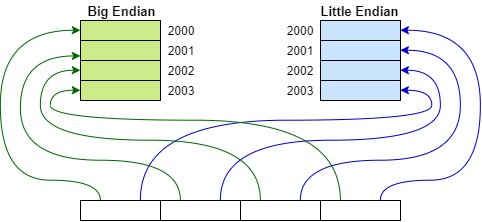
\includegraphics[scale=0.68]{Images/Programming/endians}
\caption{\footnotesize{Little Endian and Big Endian.}}
\end{figure}

The order of bytes in packets, sent through the network, is Big Endian.\\
The size of \textbf{int, float, char, ...} types
depends on the architecture used. The max size of possible types depends on the architecture (E.g. in 64bits architecture, in one istruction, 8 bytes can be written and read in parallel).

\begin{table}[h]
\centering
\begin{tabular}{|c|c|}
\hline
\textbf{signed}&{unsigned}\\
\hline
{int8\_t}&{uint8\_t}\\
{int16\_t}&{uint16\_t}\\
{int32\_t}&{uint32\_t}\\
{int64\_t}&{uint64\_t}\\
\hline
\end{tabular}\caption{<stdint.h>}
\end{table}
\vspace{4cm}
\section{Struct organization of memory}
The size of a structure depends on the order of fields and the architecture. This is caused by alignment that depends on the number of memory banks, number of bytes read in parallel. For example the size is 4 bytes for 32 bits architecture, composed by 4 banks (Figure \ref{parallel}). The Network Packet Representation is made by a stream of 4 Bytes packets as we're using 32 bits architecture. 
\begin{center}
\begin{tabular}{c}
\begin{lstlisting}[linewidth=200pt, basicstyle=\footnotesize\sffamily,]
struct example1        struct example2
{                      {
	char c;	               int x;
	int x;	               char c;
}                      }
\end{lstlisting}
\end{tabular}
\end{center}

\begin{figure}[h]
\centering
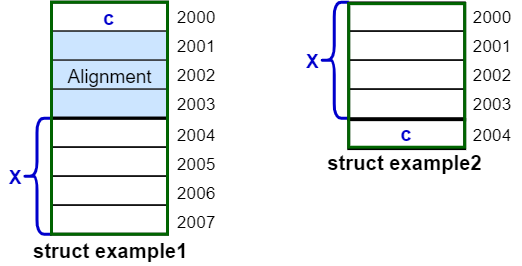
\includegraphics[scale=0.5]{Images/Programming/struct}
\end{figure}

\begin{figure}[h]
\centering
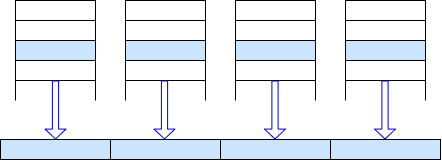
\includegraphics[scale=0.68]{Images/Programming/parallel_reading}
\caption{\footnotesize{Parallel reading in one istruction in 32 bits architecture.}}\label{parallel}
\end{figure}

\vspace{3cm}
\section{Structure of C program}
The program stores the variable in different section (Figure \ref{program}):
\begin{itemize}
\item{\textbf{Static area}\\
where global variables and static library are stored, it's initialized immediately at the creation of the program. Inside this area, a variable doesn't need to be initialized by the programmer because it's done automatically at the creation of the program with all zeroes.}
\item{\textbf{Stack}\\
allocation of variables, return and parameters of functions}
\item{\textbf{Heap}\\
dinamic allocation }
\end{itemize}

\begin{figure}[h]
\centering
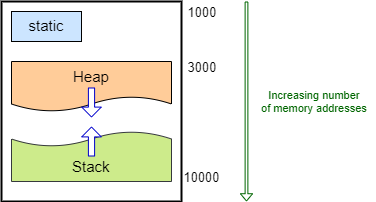
\includegraphics[scale=0.68]{Images/Programming/program}
\caption{\footnotesize{Structure of the program.}}\label{program}
\end{figure}
\chapter{Network services in C}
\section{Application layer}
We need IP protocol to use Internet. In this protocol, level 5 and 6 are hidden in Application Layer.\\
In this case, Application Layer needs to interact with Transport Layer, that is implemented in OS Kernel (Figure \ref{app_kernel}). Hence Application and Transport can talk each other with System Calls.
\begin{figure}[h]
\centering
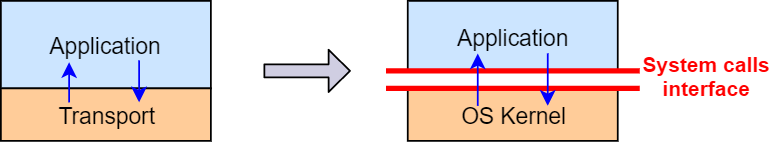
\includegraphics[scale=0.6]{Images/NetworkC/application}\caption{\footnotesize{System calls interface.}}\label{app_kernel}
\end{figure}

\section{socket}\label{socket}
Entry-point (system call) that allow us to use the network services. It also allows application layer to access to level 4 of IP protocol. 
\begin{center}
\begin{tabular}{c}
\begin{lstlisting}[linewidth=270pt, basicstyle=\footnotesize\sffamily,]
#include <sys/types.h>
#include <sys/socket.h>

int socket(int domain, int type, int protocol);\\
\end{lstlisting}
\end{tabular}
\end{center}

\begin{table}[h]
\centering
\begin{tabular}{rcl}
\textbf{RETURN VALUE} & \multicolumn{2}{l}{\textit{File Descriptor (FD) of the socket} }\\
{} & \multicolumn{2}{l}{\textit{-1} if some error occurs and errno is set appropriately}\\
{} & \multicolumn{2}{l}{(You can check value of errno including <errno.h>).}\\
\end{tabular}
\end{table}

\begin{table}[h]
\centering
\begin{tabular}{rcl}
\textbf{domain =} & \multicolumn{2}{l}{\textit{Communication domain}}\\
{} & \multicolumn{2}{l}{protocol family which will be used for communication.}\\
{} & \textbf{AF\_INET:} & {IPv4 Internet Protocol}\\
{} & \textbf{AF\_INET6:} & {IPv6 Internet Protocol}\\
{} & \textbf{AF\_PACKET:} & {Low level packet interface}\\
& &\\
\textbf{type =} & \multicolumn{2}{l}{\textit{Communication semantics}}\\
{} & \textbf{SOCK\_STREAM:} & {Provides sequenced, reliable, two-way, connection-based}\\
{} & {} & {bytes stream. An OUT-OF-BAND data mechanism may}\\
{} & {} & {be supported.}\\
{} & \textbf{SOCK\_DGRAM} & {Supports datagrams (connectionless, unreliable messages} \\
& & {of a fixed maximum length).}\\
& & \\
\textbf{protocol =} & \multicolumn{2}{l}{\textit{Particular protocol to be used within the socket}}\\
{} & \multicolumn{2}{l}{Normally there is only a protocol for each socket type and protocol}\\
{} & \multicolumn{2}{l}{family (protocol=0), otherwise ID of the protocol you want to use}\\
\end{tabular}
\end{table}

\vspace{10cm}
\section{TCP connection}
In TCP connection, defined by type \textbf{SOCK\_STREAM} as written in the Section \ref{socket}, there is a client that connects to a server. It uses three primitives (related to File System primitives for management of files on disk) that do these logic actions:
\begin{enumerate}
\item{start (open bytes stream)}
\item{add/remove bytes from stream}
\item{finish (clos bytes stream)}
\end{enumerate}
TCP is used transfering big files on the network and for example with HTTP, that supports parallel download and upload (FULL-DUPLEX). The length of the stream is defined only at closure of the stream.
 
\subsection{Client}
\subsubsection{connect}
The client calls \textbf{connect()} function, after \textbf{socket()} function of Section \ref{socket}. This function is a system call that client can use to define what is the remote terminal to which he wants to connect.

\begin{center}
\begin{tabular}{c}
\begin{lstlisting}[linewidth=370pt, basicstyle=\footnotesize\sffamily,]
#include <sys/types.h>
#include <sys/socket.h>

int connect(int sockfd, const struct sockaddr *addr,socklen_t addrlen);
\end{lstlisting}
\end{tabular}
\end{center}

\begin{table}[h]
\centering
\begin{tabular}{rcl}
\textbf{RETURN VALUE} & \multicolumn{2}{l}{\textit{0} if connection succeds}\\
{} & \multicolumn{2}{l}{\textit{-1} if some error occurs and errno is set appropriately}\\
& & \\
\textbf{sockfd =} & \multicolumn{2}{l}{\textit{Socket File Descriptor} returned by socket().}\\
& &\\
\textbf{addr =} & \multicolumn{2}{l}{\textit{Reference to struct sockaddr}}\\
{} & \multicolumn{2}{l}{sockaddr is a general structure that defines the concept of address.}\\
{} & \multicolumn{2}{l}{In practice it's a union of all the possible specific structures of each protocol.}\\
{} & \multicolumn{2}{l}{This approach is used to leave the function written in a generic way.}\\
& & \\
\textbf{addr =} & \multicolumn{2}{l}{\textit{Length of specific data structure used.}}\\
\end{tabular}
\end{table}
\vspace{8cm}
In the following there is the description of struct \textbf{sockaddr\_in}, that is the specific sockaddr structure implemented for family of protocls \textbf{AF\_INET}:

\begin{center}
\begin{tabular}{c}
\begin{lstlisting}[linewidth=350pt, basicstyle=\footnotesize\sffamily,]
#include <netinet/in.h>

struct sockaddr_in {
    sa_family_t    sin_family; /* address family: AF_INET */
    in_port_t      sin_port;   /* port in network byte order */
    struct in_addr sin_addr;   /* internet address */
};

/* Internet address. */
struct in_addr {
    uint32_t       s_addr;     /* address in network byte order */
};\\
\end{lstlisting}
\end{tabular}
\end{center}
As mentioned in Section \ref{littleBig}, network data are organized as Big Endian, so in this case we need to insert the IP address according to this protocol. It can be done as in previous example or with the follow function:
\begin{center}
\begin{tabular}{c}
\begin{lstlisting}[linewidth=280pt, basicstyle=\footnotesize\sffamily,]
#include <sys/socket.h>
#include <netinet/in.h>
#include <arpa/inet.h>

int inet_aton(const char *cp, struct in_addr *inp);
\end{lstlisting}
\end{tabular}
\end{center}
The port number is written according to Big Endian architecture, through the next function:
\begin{center}
\begin{tabular}{c}
\begin{lstlisting}[linewidth=200pt, basicstyle=\footnotesize\sffamily,]
#include <arpa/inet.h>

uint16_t htons(uint16_t hostshort);
\end{lstlisting}
\end{tabular}
\end{center}

\subsubsection{write()}
Application protocol uses a readable string, to excange readable information (as in HTTP). This tecnique is called simple protocol and commands, sent by the protocol, are standardized and readable strings.  

\begin{center}
\begin{tabular}{c}
\begin{lstlisting}[linewidth=280pt, basicstyle=\footnotesize\sffamily,]
#include <unistd.h>

ssize_t write(int fd, const void *buf, size_t count);
\end{lstlisting}
\end{tabular}
\end{center}

\begin{table}[h]
\centering
\begin{tabular}{rcl}
\textbf{RETURN VALUE} & \multicolumn{2}{l}{\textit{Number of bytes written} on success}\\
{} & \multicolumn{2}{l}{\textit{-1} if some error occurs and errno is set appropriately}\\
& & \\
\textbf{fd =} & \multicolumn{2}{l}{\textit{Socket File Descriptor} returned by socket().}\\
& &\\
\textbf{buf =} & \multicolumn{2}{l}{\textit{Buffer of characters to write}}\\
& & \\
\textbf{count =} & \multicolumn{2}{l}{\textit{Max number of bytes to write} in the file (stream).}\\
\end{tabular}
\end{table}
\vspace{4cm}
The write buffer is usually a string but we don't consider the null value (\textbf{$\backslash 0$} character), that determine the end of the string, in the evaluation of count (\textbf{strlen(buf)-1}). This convention is used because \textbf{$\backslash 0$} can be part of characters stream.\\

\subsubsection{read()}
The client uses this blocking function to wait and obtain response from the remote server. Not all the request are completed immediat from the server, for the meaning of stream type of protocol. Infact in this protocol, there is a flow for which the complete sequence is defined only at the closure of it\ref{socket}.\\
\textbf{read()} is consuming bytes fom the stream asking to level 4 a portion of them, because it cannot access directly to bytes in Kernel buffer. Lower layer controls the stream of information that comes from the same layer of remove system.\\

\begin{center}
\begin{tabular}{c}
\begin{lstlisting}[linewidth=280pt, basicstyle=\footnotesize\sffamily,]
#include <unistd.h>

       ssize_t read(int fd, void *buf, size_t count);
\end{lstlisting}
\end{tabular}
\end{center}

\begin{table}[h]
\centering
\begin{tabular}{rcl}
\textbf{RETURN VALUE} & \multicolumn{2}{l}{\textit{Number of bytes read} on success}\\
{} & \multicolumn{2}{l}{\textit{0} if EOF is reached (end of the stream)}\\
{} & \multicolumn{2}{l}{\textit{-1} if some error occurs and errno is set appropriately}\\
& & \\
\textbf{fd =} & \multicolumn{2}{l}{\textit{Socket File Descriptor} returned by socket().}\\
& &\\
\textbf{buf =} & \multicolumn{2}{l}{\textit{Buffer of characters in which it reads and stores info}}\\
& & \\
\textbf{count =} & \multicolumn{2}{l}{\textit{Max number of bytes to read} from the file (stream).}
\end{tabular}
\end{table}
So if \textbf{read()} doesn't return, this means that the stream isn't ended but the system buffer is empty.\\
If \textbf{read=0}, the function met EOF and the local system buffer is now empty. This helps client to understand that server ended before the connection.

\begin{figure}[h]
\centering
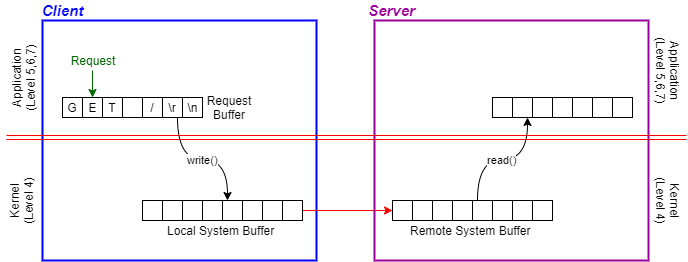
\includegraphics[scale=0.6]{Images/NetworkC/read_write1}\caption{\footnotesize{Request by the client.}}\label{rw1}
\end{figure}

\begin{figure}[h]
\centering
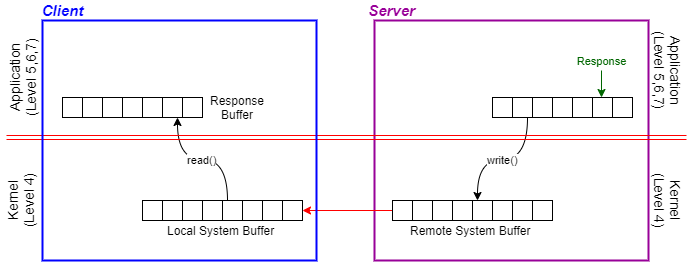
\includegraphics[scale=0.6]{Images/NetworkC/read_write2}\caption{\footnotesize{Response from the server.}}\label{rw2}
\end{figure}

\clearpage
\subsubsection{Client connection to google}
The following piece of code define a structure, used to connect to Google server. 
\lstinputlisting[caption={\footnotesize{web\_client.c}}, style=code, firstnumber=1, firstline=1, lastline=73, label=web_client, language=c]{../src/2_tcp/web_client.c}

The most important thing is that \textbf{socket()} is entry-point for level 4, but also \textbf{connect()} is the request to Kernel to extablish the connection.\\ \textbf{read()} and \textbf{write()} are system calls used respectively to obtain result(response) of a request and to generate request.\\ These function permit us to ask to lower level to do this things, without knowing content of system buffers (stream).

\section{UDP connection}
UDP connection is defined by type \textbf{SOCK\_DGRAM} as specified in Section \ref{socket}. It's used for application in which we use small packets and we want immediate feedback directly from application. It isn't reliable because it doesn't need confirmation in transport layer. It's used in Twitter application and in video streaming.  
\chapter{Shell}

\section{Commands}

\begin{table}[h]
\centering
\footnotesize
\begin{tabular}{|l|l|l|}
\hline
\multicolumn{2}{|l|}{\multirow{2}{*}{\textbf{man} man}}&{Shows info about man command and}\\
\multicolumn{2}{|l|}{} & {lists all the sections of the manual.}\\
\hline
\multicolumn{2}{|l|}{\textbf{strace} objFile} & {Lists all the system calls used in the program.}\\
\hline
\multicolumn{2}{|l|}{\textbf{gcc} -o objFile source \textbf{-v}} & {Lists all the path of libraries and headers used in creation of objFile.}\\
\hline
\multirow{3}{*}{\textbf{netstat}} & {-t} & {Lists all the active TCP connections showing domain names.}\\
\cline{2-3}
& {-u} & {Lists all the active UDP connections showing domain names.}\\
\cline{2-3}
& {-n} & {Lists all the active, showing IP and port numbers.}\\
\hline
\multicolumn{2}{|l|}{\textbf{nslookup} domain} & {Shows the IP address related to the domain (E.g. IP of www.google.it)}\\
\hline
\multicolumn{2}{|l|}{\multirow{5}{*}{\textbf{dig} @server name type}}&{DNS lookup utility.}\\
\multicolumn{2}{|l|}{}&{\textbf{server} name or IP address of the name server to query}\\
\multicolumn{2}{|l|}{}&{\textbf{name} name of the resource record that is to be looked up}\\
\multicolumn{2}{|l|}{}&{\textbf{type} type of query is required (ANY, A, MX, SIG, etc.)}\\
\multicolumn{2}{|l|}{}&{$\;\;\;\;\;\;\;\;\;\;$if no type is specified, A is performed by default}\\
\hline
\multicolumn{2}{|l|}{\multirow{2}{*}{\textbf{wc} [file]}} & {Prints in order newlines, words, and bytes (characters) counts for file}\\
\multicolumn{2}{|l|}{} & {if file not specified or equal to -, counts from stdin.}\\
\hline
\multicolumn{2}{|l|}{\multirow{2}{*}{\textbf{route} -n}} & {Show numerical addresses instead of trying to determine symbolic}\\
\multicolumn{2}{|l|}{} & {hostnames in routing table.}\\
\hline
\end{tabular}
\end{table}


\section{UNIX Files}\label{files}
\begin{table}[h]
\centering
\footnotesize
\begin{tabular}{|l|l|}
\hline
\textbf{/etc/hosts} & {Local resolution table.}\\
\hline
\multirow{2}{*}{\textbf{/etc/services}} & {List all the applications with their port}\\
& {and type of protocol (TCP/UDP).}\\
\hline
{\textbf{/etc/protocols}} & {Internet protocols.}\\
\hline
{\textbf{/usr/include/x86\_64-linux-gnu/bits/socket.h}} & {List all the protocol type possible for socket.}\\
\hline
{\textbf{/usr/include/x86\_64-linux-gnu/sys/socket.h}} & {Definition of struct sockaddr and specific ones.}\\
\hline
\end{tabular}
\end{table}

%\section{Usefull information about shell}
\end{document}